\documentclass{mybook}
\newcommand{\MA}{\mat{A}}
\newcommand{\MI}{\mat{I}}
\newcommand{\MW}{\mat{W}}
\newcommand{\Va}{\Vec{a}}
\newcommand{\Vy}{\vec{y}}
\newcommand{\Vx}{\vec{x}}
\newcommand{\Ve}{\vec{e}}
\newcommand{\Vw}{\vec{w}}
\newcommand{\Vt}{\vec{\theta}}
\newcommand{\SR}{\mathcal{R}}
\newcommand{\DN}{\mathcal{N}}


\addbibresource{main.bib}
\begin{document}

\title{《交通数据分析》讲义}
\author{熊耀华}
\date{2023年01月02日}
\maketitle
\tableofcontents

\part{本科课程}

%重定义放在mycommand.tex里面无效,为什么?
\renewcommand{\vec}[1]{\symbfit{#1}}

\chapter{绪论:交通和数据}
\begin{cabstract}
    \item 数据是证据
    \item 交通中有哪些常见数据
    \item 数据处理是转化数据得到信息
\end{cabstract}

当前人类文明已经进入了所谓的“信息时代”,数据已经渗透进我们社会生产、生活的方方面面,交通领域也不例外。
作为一门工程学科,交通领域的相关专业,如交通工程、交通运输、交通安全等,都遵循“发现问题、分析问题解决问题”的逻辑步骤,在每一个步骤数据都发挥决定性的作用。
本章对交通和数据的关系进行概括的介绍。

\section{什么是数据?}

“\emph{数据}”这个词我们在日常生活中已经广泛使用,但它的来源和确切含义却并不广为人知。
事实上这个词语具有丰富的内涵,了解它不只是满足我们的好奇心,更是让我们能真正意识到它的\emph{重要意义}。中文的“数据”一词翻译自英文单词“data”,按照《牛津字典》的解释,它至少包含两层含义:
\begin{itemize}
    \item 计算机可以操作的数值、字母、符号,能够以磁、光、电、机械的形式存储和传输。
    \item 假设成立或验证成立的\emph{事实},作为进一步推理和计算的基础。\sidenote{things known or assumed as facts, making the basis of reasoning or calculation.}
\end{itemize}
可以看到第一层含义更贴近我们日常用语习惯,但第二层含义才是“data”这个单词的真正来源。

\begin{marginfigure}

\includegraphics[width=\linewidth]{images/spqr.png}
\caption{SPQR(Senatus PopulusQue Romanus)——罗马元老院和人民。}
\end{marginfigure}

英文单词“data”来源于\emph{拉丁语}%
\sidenote{拉丁语是古罗马文明的语言,是意大利语、西班牙语、法语的祖先。罗马帝国灭亡后在很长时间内,拉丁语仍然是欧洲各国进行宗教、文化、科技交流的通用语言。}%
这门古老的语言,原型是拉丁语动词原型“dare”,英文翻译“to give”,意为“给”;按照语法,“dare”的被动语态分词是“datum”,英文翻译为“to be given”,意为“被给”;进一步分词名词化,“datum”可以解释为“thing to be given”,意为“被给的东西”。
17世纪中期欧洲哲学家开始在著作中用“datum”一词表达讨论中已经“\emph{给定(given)}”的前提条件,在拉丁语中“datum”作为名词是中性单数,因此对应的复数形式就是“data”。

从来源可以看出,“data”一词实际上是一个哲学概念,是我们探索未知的已知基础。
他的形式并不局限于数字,可以以任何方式存在,例如文字、图片、符号等等;他的重要性和广泛性也远超越交通领域、甚至远远超越了工程技术、自然科学,进入人文、艺术、哲学范畴,
因此一经问世快速被各个领域的学者采纳。
该词汇在书籍中使用比例的变化情况如\cref{fig:data-trend}所示。
当然,随着计算机技术的发展各种“data”的表示方式逐渐\emph{数字化},因此如今我们可以把“数据”理解为以数字形式存在的\emph{证据}。

\begin{figure*}
    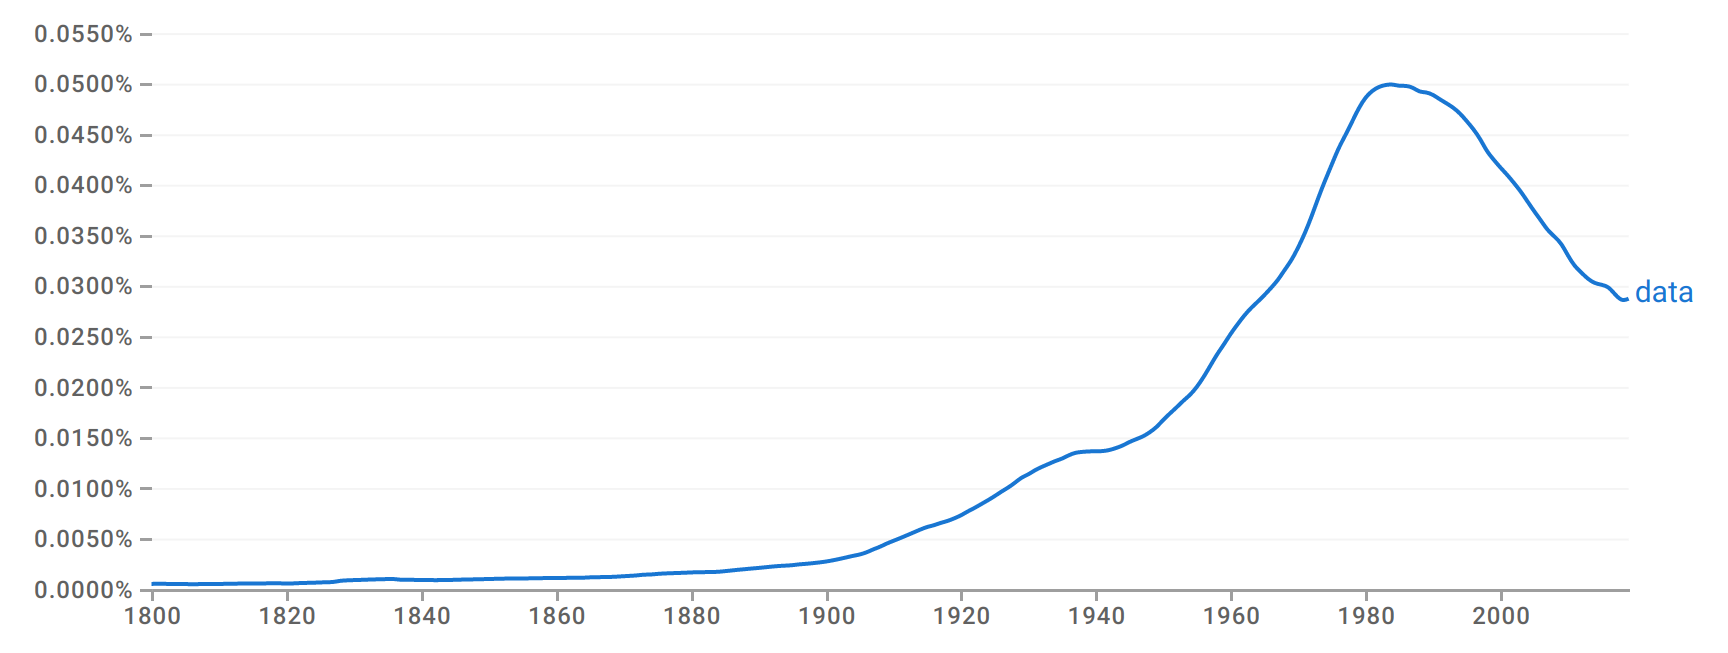
\includegraphics[width=\linewidth]{images/data-vocabulary-trend.png}
    \caption{英文书籍中单词“data”使用频率的变化,数据来自Google Book}
    \label{fig:data-trend}
\end{figure*}

\section{交通数据}

交通数据是指与交通系统的规划、设计、运营、控制相关的数据,是研究交通系统运行规律,解决现实交通问题的基础。本节概括介绍常见交通数据的类型、用途、获取方式。

交通最基本的定义是人和货物的移动;\emph{交通系统}是指人、货物、以及参与他们移动的其他要素的总和。
交通系统是由大量、相互作用的要素构成的复杂系统,为方便分析需要划分更小的子系统,由于交通系统的复杂性有多种划分标准,以下是几个例子:
\begin{itemize}
    \item 按照交通主体划分,可以分为客运交通和货运交通。
    \item 按照城市范围划分,可以分为市区交通和市郊交通,分别有不同的管理方式。
    \item 按照交通方式划分,某个区域的交通网络由道路、轨道、航空、水运、管道等子系统构成,分别有不同的技术特征、运营方式、适用条件。
    \item 按照经济角色划分,可以分为\emph{交通供应}和\emph{交通需求}两个部分,分别有不同的利益诉求\sidenote{例如供应方公交公司希望通过降低发车间隔来降低成本,需求方乘客希望增加发车间隔来减少等待时间}。
\end{itemize}
实际对交通系统的划分可以更加复杂。例如可以把以上三个标准任意组合,得到新的划分标准;也可以对划分后的子系统进一步划分。这里为了控制课程范围我们主要关注市区内基于道路和轨道的客运交通,简称\emph{城市交通}。该领域通常关注的数据将在以下小节分别介绍。

\subsection{路段交通状态数据}

路段交通状态数据是指路网中某个路段在某个时刻的交通流量、密度、速度数据,简称流密速数据。
简单来说,流量是单位时间通过给定道路断面的车辆数;密度是单位长度路段上某瞬间的车辆数;速度是指某个时间、空间范围内所有车辆轨迹的\emph{平均}速度。
路段是交通网络的最小组成部分,描述单个路段交通状态是分析整个路网交通状态的基础。

\subsubsection{流量调查}
路段流量数据的获取方式最简单,只需在路段某个位置记录通过车辆的数量。
传统方法是由调查人员在路边人工数车,这种方法的好处是不需要任何技术装备,因此2000年以前应用广泛。
人工调查的缺点是受人力成本的限制,调查规模小、数据采集速度慢、且难以做到全天侯全时段采集。

\begin{marginfigure}
    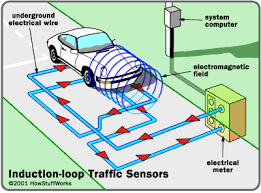
\includegraphics[width=\linewidth]{images/induction-loop-sensor.png}
    \caption{感应线圈检测器工作原理}
    \label{fig:induction-loop}
\end{marginfigure}

当前流量调查的主流方式时感应线圈检测器。该设备需要在路段地下埋设通电金属线圈,然后通过记录车辆压过线圈时产生的电磁感应电流脉冲来检测车辆,原理见\cref{fig:induction-loop}。该设备现在技术成熟、价格经济,已经普及到大城市的多数重要道路,成为最重要的交通数据来源。

\subsubsection{速度调查}

速度调查一般分为两个阶段,首先是单个车辆瞬时速度调查,然后是根据多个车辆的瞬时速度计算路段平均速度。单个车辆瞬时速度调查可以直接用测速枪,发射声波或电磁波,通过车辆反射波的多普勒效应推算车辆速度如\cref{fig:speed-gun}所示。
也可以用双断面法,测量车辆通过两个相邻断面的时间差,然后除以断面之间距离差来得到速度,如\cref{fig:section-speed}所示。

\begin{marginfigure}
    
\includegraphics[width=\linewidth]{images/speed-gun.jpg}
    \caption{测速枪测速。}
    \label{fig:speed-gun}
\end{marginfigure}

\begin{marginfigure}
    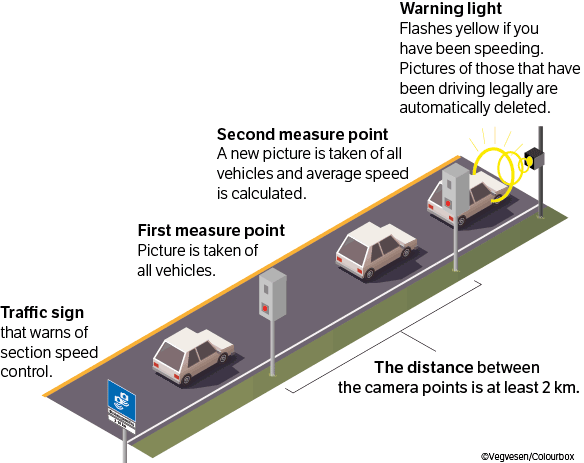
\includegraphics[width=\linewidth]{images/section-speed.png}
    \caption{双断面法测速。}
    \label{fig:section-speed}
\end{marginfigure}

\subsubsection{密度调查}
交通密度传统上一般难以直接调查,需要基于流量和速度间接推测。
交通密度直接调查需要进行高空俯视拍照,然后用照片范围内的车辆数除以路段长度就能得到交通密度。
为了保证照片的视野范围,拍摄站位一般需要飞机、热气球、高楼顶等高处,而实际上往往找不到合适位置,因此不可行。
另一方面流密速三者之间存在函数关系$q=k\cdot v$,同时流量$q$和速度$v$都比较容易获取,因此实际应用中一般通过$k=\frac{q}{v}$来推算密度。

\begin{figure}
    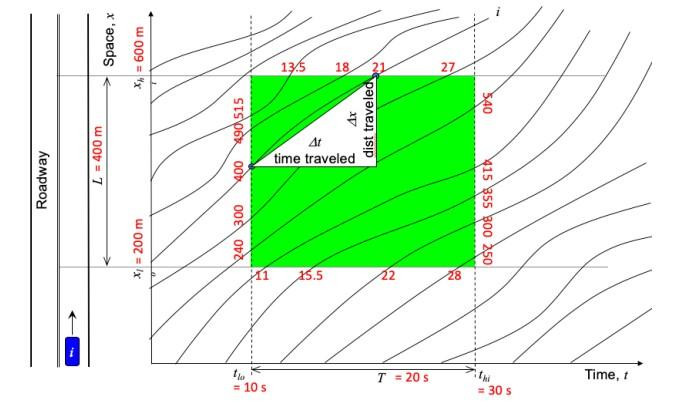
\includegraphics[width=\linewidth]{images/flow-density-speed.jpeg}
    \caption{路段车辆轨迹图;流量、密度、速度可以从轨迹推算。}
    \label{fig:trajectory}
\end{figure}
\subsection{车辆轨迹数据}
车辆轨迹数据又称车辆时空轨迹数据,是车辆时空位置记录构成的序列。每条记录记录包含两个成分,时间点和该时间点时车辆的空间位置;所有记录按时间点由早到晚排序。
一条车辆轨迹描述了某一车辆的完整活动轨迹,而车辆又是道路交通的最小单位,采集所有车辆的轨迹理论上可以掌握道路交通系统的完整状况。与路段流密速数据相比,车辆轨迹数据包含更加丰富的信息。从轨迹数据可以推算出流密速,反之则不成立,见\cref{fig:trajectory}。

车辆轨迹数据包含时间和位置两个成份,其中时间信息通过计时设备获取,比较简单,难点主要在空间位置信息的获取。
主要方式可以归纳为两类:路标定位和三角定位。

\subsubsection{固定信标定位}
设想你乘船在漆黑的大海上航行,如何获取自己的位置。
最简单的方法是去最近的灯塔,询问灯塔上的看守者。看守者知道自己灯塔的位置,你在这个灯塔附近因此也知道了自己的位置。在这个场景里灯塔这种位置已知的标记就是\emph{信标}。

在城市交通场景中可以承担信标角色的主要是固定的车辆身份识别设备,例如电子警察、ETC卡口等。
有车辆经过时这些设备能记录下车辆的身份、通过时间。
获取大量记录之后可以把某一辆车通过的卡口编号按时间顺序排列,然后将卡口编号替换为卡口位置,从而得到车辆的时空轨迹。
这种方法的核心是需要区分车辆的身份%
\sidenote{近年来兴起的所谓车路通信设备可以通过乘客手机上的蓝牙、Wifi信号区分乘客身份,进而间接区分车辆身份,因此也能作为固定信标。}%
,以免不同车辆的记录混淆,因此无法区分车辆身份的线圈检测器不能作为信标。

\subsubsection{三角定位}
固定信标定位简单易行,但有一个不足:只有到达信标附近才能用信标的位置来定位。
仍然以大海中的中的航船为例,航线中经过灯塔的时间和位置可以确定,而灯塔之间的实际航行路线无法确定,只能假设为直线。
要在不靠近灯塔的情况下确定船只位置需要用到附近至少三个灯塔,同时假设每个灯塔的位置已知,且有某种手段能测量船只和灯塔的距离。
每个灯塔的位置和距离把船只限定在一个灯塔的同心圆上,而三个灯塔同心圆的交点就是船只的位置。
这种获取位置的方法称为三角定位法,如\cref{fig:triangle-localization}所示。
\begin{marginfigure}
    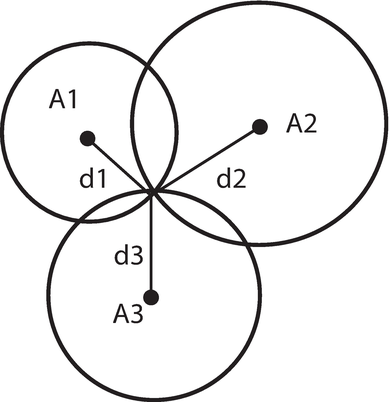
\includegraphics[width=\linewidth]{images/triangle-localization.png}
    \caption{三角定位法用三个固定信标推测当前位置。}
    \label{fig:triangle-localization}
\end{marginfigure}

在城市交通中常用的定位方式如卫星定位、手机基站定位本质上都是三角定位,只是担任信标角色的不是灯塔而是卫星和手机基站。
当前有几套卫星定位系统同时运行,包括美国的GPS系统、欧洲的伽利略系统、中国的北斗系统;其中GPS系统历史最长、覆盖范围最广。
几套系统的基本原理相似,天空中的卫星以固定轨道运行,位置已知,担任信标。
卫星持续向地面发射信号,信号中包含持续更新的高精度时间信息。
地面的定位设备接收卫星信号,比较信号的发射时间和接收时间,时间差乘以电磁波速度得到定位设备与卫星的距离。

手机基站定位原理类似,只不过用手机基站取代卫星作为电磁波发射源。
与卫星定位相比手机基站定位的精度低,而且只能在有手机信号的区域工作,覆盖范围窄。
但卫星定位与手机基站定位的最大区别在于前者是一种\emph{分散式}的数据采集手段,而后者是一种\emph{中心化}的数据采集手段。
设想我们要采集成都市所有人每天的活动轨迹。如果采用卫星定位技术,虽然现在所有手机都支持卫星定位但是我们很难让每一个手机用户都同意上传他的实时位置
\sidenote{现在有不少手机App会上传卫星定位数据到背后公司的数据库,如各种导航、点评、社交软件。}。
与之相对的是,如果采用手机基站定位,理论上只要运营商配合,不需要征得手机用户的同意就能获取成都所有人的实时位置。

\subsection{道路网数据}
道路网是城市交通最重要的基础设施,道路网数据是分析城市交通系统的基础数据。
道路网数据是城市地图数据的组成部分,一般包括道路平面位置和线型、车道划分、交叉口位置、交叉口渠化、交叉口信号控制方案等信息。
传统上道路数据的收集和处理主要属于地理信息专业,但现在随着智能交通的发展在交通专业中也越来越重要。

获取数字地图数据的方法主要是通过航拍、卫星图等方式获得某个区域的大范围照片,然后利用专业GIS软件在照片上描绘道路、房屋,并将各种信息输入数据库,如\cref{fig:gis-data-collection}所示。
传统上描绘过程需要人工操作,近年出现自动完成描绘的技术。
\begin{figure*}
    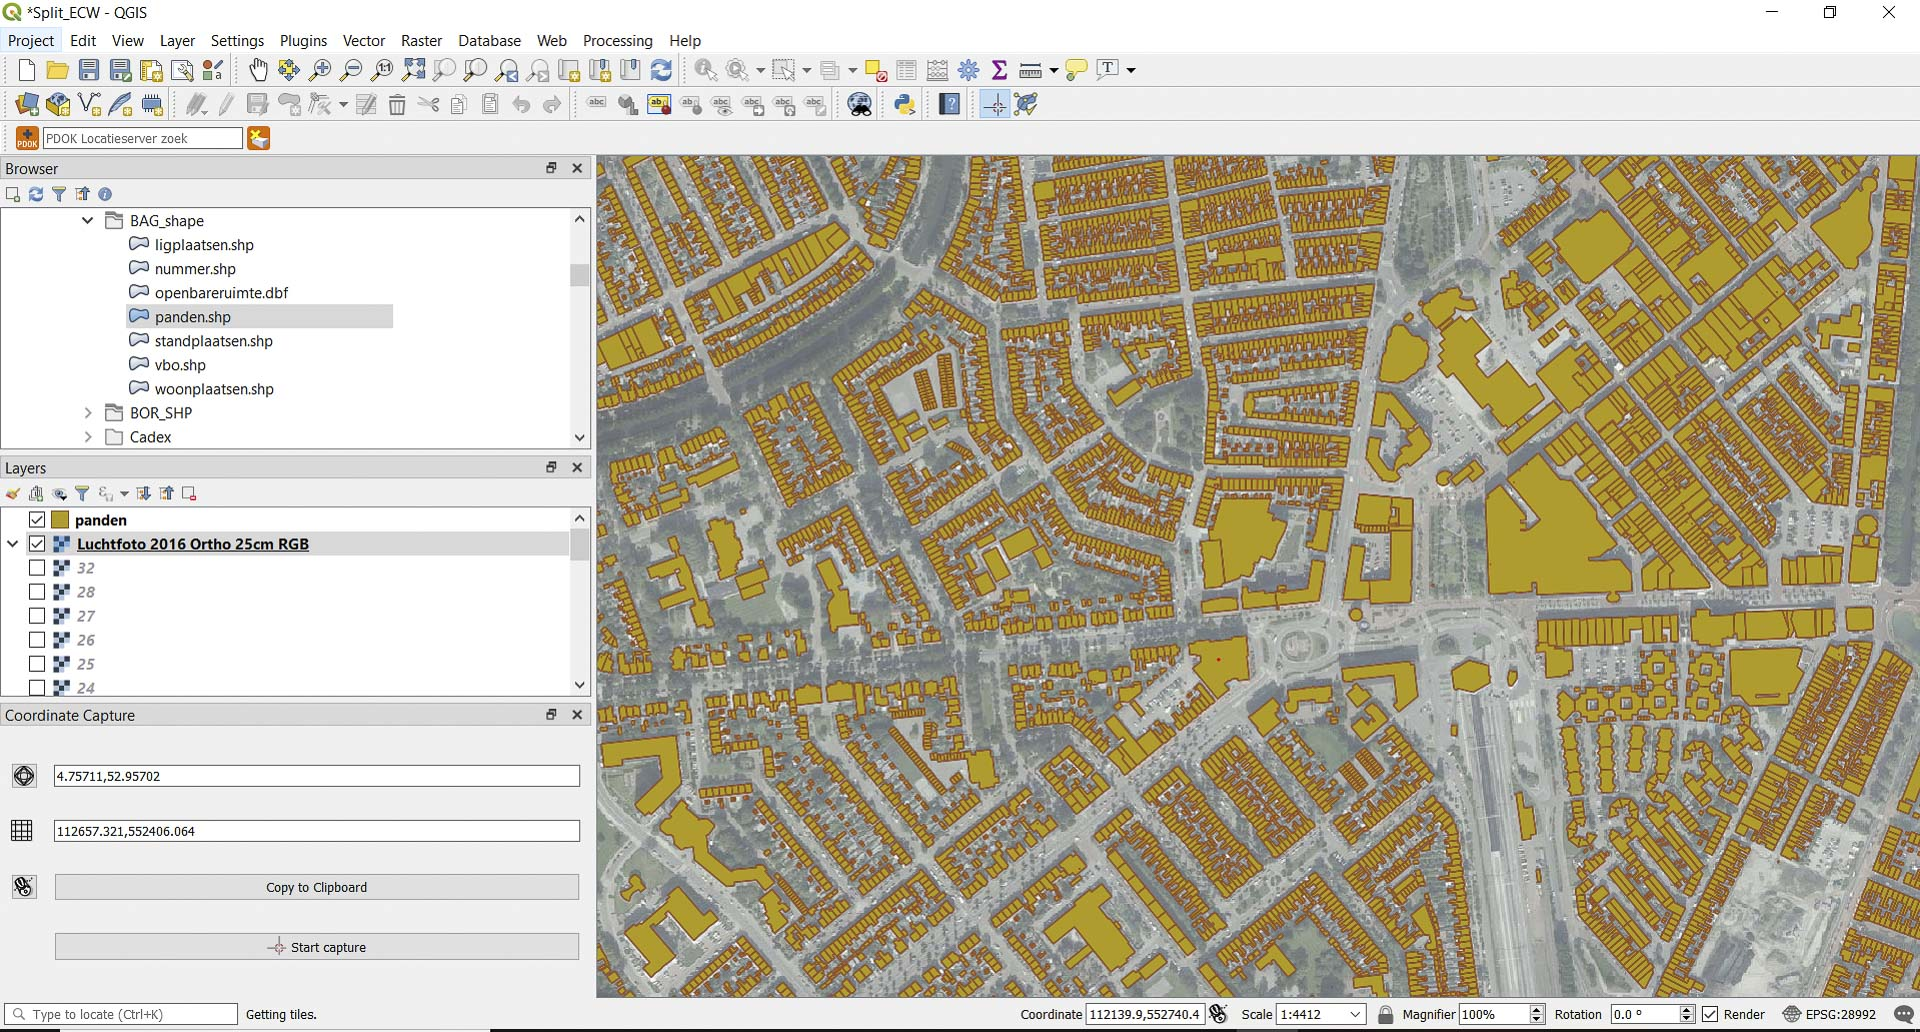
\includegraphics[width=\linewidth]{images/gis-data-collection.jpg}
    \caption{用QGIS软件处理卫星照片,建立数字地图数据}
    \label{fig:gis-data-collection}
\end{figure*}

\subsection{出行者行为数据}
之前的数据描述的是交通系统的状况,但解决交通问题往往需要探寻造成某种状况背后的原因。
决定交通系统状况最根本的原因是出行者的\emph{选择行为}。
每个出行者每天都面临着大到在什么地方买房定居、小到开车快慢的无数选择;
一个城市中所有出行者的所有选择共同决定了城市交通系统的状态。
例如大量出行者选择走某条道路会造成该道路拥堵,大量出行者同时去某个区域会造成该区域停车困难。

理解选择行为需要用到经济学模型,这些模型需要的数据包括出行者的社会经济背景,例如性别、年龄、收入、教育程度;各种偏好,例如时间和钱的兑换比例。这些数据一般通过问卷调查获取。

\section{什么是数据处理}

从各种渠道获取的数据称为\emph{原始数据},质量可能参差不齐,形式可能不符合要求,也可能太过繁杂难以抓住重点,因此需要经过处理才能变成有效的信息。
而\emph{数据处理}就是指用一切方法对数据进行变换,直到得到有效信息的过程。

数据处理的环节根据不同应用的要求多种多样,但以下这些环节比较常见。

\begin{description}
    \item[验证] 原始数据根据来源不同质量可能有很大差别。拿到数据后的第一步一般是验证数据质量,发现缺失、重复、错误、自相矛盾等问题,并力所能及的修正。如果修正不了至少要掌握误差的程度。
    \item[融合] 不同来源的数据往往有不同的形式,数据融合是将不同形式的数据统一到一个形式,方便后续使用。
    \item[统计] 大量细节数据容易造成信息过载,让人抓不住重点。通过统计手段可以将数据浓缩到少量关键值,例如均值、方差等,方便理解。
    \item[建模] 数据本身只反映出现象,重要的是探索现象背后的机理。综合利用各种数学工具可以建立数学模型,解释数据之间的关系,发现背后的机理。
    \item[可视化] 将数据从抽象的数字形式转化为图片、动画等可见的形式,利用人类视觉理解能力。通过可视化不只是方便展示数据处理的最终结果,更重要的是帮助发现数据中隐藏规律。
\end{description}

\chapter{数据模型初探}

数据本身只反映出现象,因此我们的目的不仅仅是搜集数据本身,而是通过数据发现背后的机理和规律——
不只是回答“怎么样”,更重要的是回答“为什么”。而发现数据中规律的重要方法就是数据模型。

\section{交通流模型}

以一条道路上的交通状态为例,我们可以用流量$q$、密度$k$、速度$v$三个指标来描述。
其中根据物理守恒定律很容易推导出$q=k\cdot v$,另一方面密度$k$和速度$v$之间的关系就不是那么直观了。对于这种未知的关系,我们可以用一个函数$v=f(k)$表示,$f$的数学定义就代表了速度和密度之间的关系,也是路段上交通状态变化的背后机理。

为了找出合适的函数$f$我们要从实际出发,首先通过各种手段实际观测道路上的流量、密度、速度。
直接从现实世界观测到的数据称为\emph{实测数据(empirical data)}%
\sidenote{empirical是一个哲学词汇,反义词是ideological。分别表示基于现实世界的的和基于意识形态的证据}
,大量数据如果以数字表格形式存在,我们很难理解。
因此第一步一般是将数据可视化,绘制成某种图形。

路段流密速数据一般可视化方法是以将每一条记录画作一个数据点,横坐标表示密度、纵坐标表示速度或流量。实测数据绘制后一般呈现出类似\cref{fig:empirical-qkv}的形态,从中马上可以看出一些规律。
例如从左图中速度和密度之间的关系,可以看出随着密度增加速度总体呈下降趋势;而且密度较小时速度下降不明显。从右图中流量和密度之间的关系,可以看出随着密度增加流量呈先上升后下降的趋势。

\begin{figure*}
    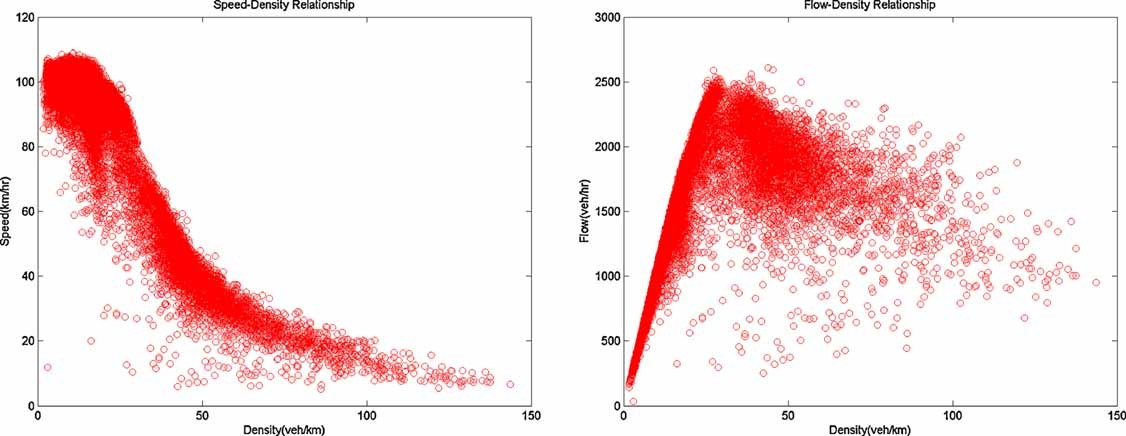
\includegraphics[width=\linewidth]{images/empirical-qkv.jpg}
    \caption{路段流量、密度、速度的典型实测数据}
    \label{fig:empirical-qkv}
\end{figure*}

由于我们已经知道$q=k\cdot v$,也就是说知道$k$,$v$就能计算出$q$,因此流量$q$对于我们来说是\emph{冗余数据(redundant data)},在后续分析中可以舍弃\sidenote{冗余数据并非没有价值,可以用于验证数据有效性。这里直接舍弃是为了简化讨论。}。此时我们面临的问题是,定义一个函数
\begin{equation}
    v=f(k)
\end{equation}
让该函数的图像与实测数据尽量符合,在数学上称为\emph{拟合问题}。

为了确定函数$f$的定义我们需要回答两个问题。第一个问题是函数的基本形态是什么?例如是直线、抛物线、还是指数曲线。这里我们假设$f$的图像是一条直线\sidenote{合理选取函数形式要综合考虑很多因素,没有标准答案,需要结合经验和对数据本身的理解。}
,也可以说$f$是\emph{线性函数}。
对于线性函数我们可以写出公式
\begin{equation}\label{eq:linear-kv}
    v = a\cdot k + b
\end{equation}
其中$a$和$b$是未知\emph{参数(parameter)}。
解析几何告诉我们$a$,$b$参数取值决定直线的形态,因此第二个个问题是$a$、$b$取值多少函数$f$与实测数据吻合\emph{最好}。

\section{线性回归}
为了确定\cref{eq:linear-kv}中的参数$a$、$b$我们需要用到一种叫做\emph{线性回归}的数学方法。
不过在正式介绍线性回归前,我们可以看一个简化的例子,方便理解为什么需要线性回归。

\subsection{线性方程}

假设我们实测的数据只有两组,即两个不同时刻的密度和速度,分别写作$p_1\coloneqq(k_1, v_1), p_2\coloneqq(k_2, v_2)$\sidenote{数学符号$\coloneqq$表示两边定义等价,读作“定义为”。}
,其中$p$代表数据点(point)。
此时图上只有两个数据点,函数$f$的图像是一条直线,显然当它同时穿过$p_1$、$p_2$时对数据的拟合最好。如何确定此时$a$、$b$的取值?

我们可以通过线性方程组来求解$a$、$b$。由于直线穿过两个数据点,以下两个方程必定成立:
\begin{equation}
    \left\{
    \begin{aligned}
        v_1 &= a\cdot k_1 + b \\
        v_2 &= a\cdot k_2 + b
    \end{aligned}\right.
\end{equation}
其中$a$、$b$是需要求解的未知数,可以用高斯消元法求解。
但这里我们先不求解,而是先把方程组写成线性代数的形式,方便后面的讨论。
首先将未知数写成单独分离,得到
\begin{equation}\label{eq:la-kv}
    \begin{bmatrix}
        v_1\\
        v_2
    \end{bmatrix}=
    \begin{bmatrix}
        k_1 & 1\\
        k_2 & 1
    \end{bmatrix}\cdot
    \begin{bmatrix}
        a\\
        b
    \end{bmatrix}
\end{equation}

可以看到方程由三项构成,我们分别规定用字母表示。其中左边是所有速度数据构成的向量%
\sidenote{注意区别$\Vv$和$v$,黑体字母$\Vv$表示向量,正常字母$v$表示标量。}
,写作$\Vv$;中间是一个权重(weight)矩阵,写作$\MW$;右边是由所有参数构成的矩阵,写作$\Vu$。此时\cref{eq:la-kv}进一步简化表示为
\begin{equation}
    \Vv=\MW\cdot\Vu
\end{equation}
如果权重矩阵$\MW$可逆,参数$a$、$b$可以通过以下公式计算
\begin{equation}\label{eq:la-eq}
    \begin{bmatrix}
        a\\
        b
    \end{bmatrix}=
    \Vu=\MW^{-1}\cdot\Vv
\end{equation}
而这里的权重矩阵$\MW=\big[
\begin{smallmatrix}
    k_1 & 1\\
    k_2 & 1
\end{smallmatrix}$\big]
是$2\times2$的正方形矩阵,一般来说可逆。

\subsection{最小二乘法}

现在我们重新做了一次测量,得到一组新的数据$p_3\coloneqq(k_3, v_3)$,此时问题的性质发生了变化。按照上一节的步骤我们得到线性方正组
\begin{equation}\label{eq:la-kv-3}
    \begin{bmatrix}
        v_1\\
        v_2\\
        v_3
    \end{bmatrix}=
    \begin{bmatrix}
        k_1 & 1\\
        k_2 & 1\\
        k_3 & 1
    \end{bmatrix}\cdot
    \begin{bmatrix}
        a\\
        b
    \end{bmatrix}
\end{equation}
但是此时权重矩阵的尺寸是$3\times2$,一般来说不可逆,无法求解$a$,$b$。
无法求解的原因是我们有两个未知量$a$、$b$,但是有三个约束条件分别来自数据$p_1$、$p_2$、$p_3$,这类问题在数学上称为\emph{过约束}问题。

线性回归是解决这类过约束问题的常见方法,能够在没有精确解的情况下求出最优近似解。
当线性方程组$\Vv=\MW\cdot\Vu$因为过约束无解时,方程两边同时乘以$\MW^{-1}$,将\cref{eq:la-eq}转化为以下\emph{最小二乘形式}
\begin{equation}\label{eq:least-square}
    \MW^{-1}\Vv=\MW^{-1}\MW\cdot\Vu
\end{equation}
此时方程是否有解由矩阵$\MW^{-1}\MW$是否可逆决定。
可以证明无论$\MW$是什么形状,$\MW^{-1}\MW$都是正方形矩阵,一般来说可逆。
为了与精确解区别,最佳近似解记作$\Vu^*$,可以通过以下公式计算
\begin{equation}
    \Vu^*=(\MW^{-1}\MW)^{-1}\MW^{-1}\Vv
\end{equation}

\section{线性回归原理}

\cref{eq:least-square}中我们直接给出了线性回归求解最佳近似解的方法,本节将解释为什么这个公式有效。要理解线性回归的原理,有代数和几何两个角度。其中代数角度的关键是残差平方和最小,几何角度的关键是向量空间的正交投影。以下将分别解释。

\subsection{残差平方和最小}
假定参数$a$,$b$为已知量,利用\cref{eq:linear-kv}可以根据密度$k$计算速度$v$。
此时一个密度对应两个速度,一个称为\emph{实测值}另一个称为\emph{预测值}。
例如密度$k_1$对应的实测值是$v_1$,预测值为了区别记作$\hat{v}_1=f(k_i)=ak_1+b$。
\nolinebreak\sidenote[][0cm]{$\hat{v}$读作“hat v”或者“帽子 v”}%
实测值和预测值之间的差别称为\emph{残差},记作$e_1=\hat{v}_1-v_1$。
理想情况下实测值与预测值吻合,残差$e_1=0$;如果做不到,越接近$0$越好。

\subsubsection{残差平方和}

当有多个数据点时,我们需要一个指标表示所有数据点预测值和估计值的总体吻合程度,常用的指标\emph{残差平方和(Sum of Squares Error)}定义为:
\begin{equation}\label{eq:sse}
    \text{SSE}=\sum_{i=1}^n {e_i}^2=\sum_{i=1}^n (v_i-f(k_i))^2
\end{equation}
其中$n$是数据点数量,$e_i$代表第$i$个数据点的残差。残差平方和并不是唯一的指标,首先介绍的原因是他有一些良好的性质,可以简化数学处理。
另一个常用的指标是\emph{残差绝对值之和}$\sum_{i=1}^{n}|e_i|$,虽然在数学处理上难度更高,但是在其他方面更有优势,会在后续章节介绍。

根据以上定义可以看出残差平方和$\text{SSE}$是参数$a$、$b$的函数,因为不同的$a$、$b$取值会影响预测值$\hat{v}$,进而影响到残差$e_i$,再而影响到残差平方和。需要特殊强调这个函数关系时残差平方和可以记作$\text{SSE}(a,b)$或者$\text{SSE}(\Vu)$,接下来我们推导它的公式。

根据\cref{eq:sse}的定义,我们可以把残差平方和写成向量\emph{点积}形式
\begin{equation}\label{eq:sse-vec}
    \begin{split}
        \text{SSE}&=\sum_{i=1}^n {e_i}^2=
        \begin{bmatrix}
            e_1 & e_2 &\cdots & e_n
        \end{bmatrix}
        \cdot
        \begin{bmatrix}
            e_1 \\
            e_2 \\
            \vdots\\
            e_n
        \end{bmatrix}\\
        &=\Ve^T\cdot\Ve
    \end{split}
\end{equation}
其中$\Ve=[\begin{smallmatrix}
    e_1 & e_2 & \cdots & e_n
\end{smallmatrix}]^T$是所有残差构成的列向量。
接下来我们写出残差向量$\Ve$的公式
\begin{equation}\label{eq:e-vec}
    \begin{split}
        \Ve=
        \begin{bmatrix}
            e_1 \\
            e_2 \\
            \vdots\\
            e_n
        \end{bmatrix}&=
        \begin{bmatrix}
            v_1 \\
            v_2 \\
            \vdots\\
            v_n
        \end{bmatrix}-
        a\cdot
        \begin{bmatrix}
            k_1 \\
            k_2 \\
            \vdots\\
            k_n
        \end{bmatrix}-
        b\cdot
        \begin{bmatrix}
            1 \\
            1 \\
            \vdots\\
            1
        \end{bmatrix}\\
        &=\Vv-a\Vk-b\vec{1}\\
        &=\Vv-\MW\Vu
    \end{split}
\end{equation}
其中$\Vv$是所有速度实测值的向量,$\MW$是权重矩阵,$\Vk$是所有密度数据的向量,$\vec{1}$是全$1$向量。

把\cref{eq:e-vec}带入\cref{eq:sse-vec},然后展开化简可以得到
\begin{equation}\label{eq:sse-function}
    \begin{split}
        \text{SSE}(\Vu) &= \Ve^T\cdot\Ve\\
        &=(\Vv-\MW\Vu)^T(\Vv-\MW\Vu)\\
        &=\Vv^T\Vv+(\MW\Vu)^T\MW\Vu
        -\Vv^T\MW\Vu-(\MW\Vu)^T\Vv\\
        &=\Vv^T\Vv+(\MW\Vu)^T\MW\Vu
        -(\MW\Vu)^T\Vv-(\MW\Vu)^T\Vv\\
        &=\Vu^T\MW^T\MW\Vu-2\Vu^T\MW^T\Vv-\Vv^T\Vv
    \end{split}
\end{equation}
其中我们用到向量点积的交换关系$\Va^T\Vb=\Vb^T\Va$,以及矩阵转置的交换关系$(\MA\MB)^T=\MB^T\MA^T$。

\subsubsection{残差平方和最小化}

通过推导我们写出了残差平方与参数之间公式$\text{SSE}(\Vu)$,接下来就是要找到特定的参数取值$\Vu=\Vu^*$,让$\text{SSE}(\Vu^*)$最小;
即$\text{SSE}(\Vu^*)\leq\text{SSE}(\Vu)\text{,}\forall\Vu$。
这是一个典型的\emph{最优化问题},可以记作
\sidenote{$\argmin$是“argumentum minimi”,最小化参数,的缩写;与之对应的是$\argmax$,“argumentum maximi”。}
\begin{equation}
    \Vu^*=\argmin \text{SSE}(\Vu)
\end{equation}

观察\cref{eq:sse-function},可以看到$\text{SSE}(\Vu)$的自变量$\Vu$虽然是向量,但是总体形式类似于一个抛物线函数$au^2-bu+c$。
利用微积分的知识,我们推测该函数存在最小值,且最小值处导数为$0$。由此我们列出方程
\begin{equation}
    \begin{split}
        \frac{\partial\text{SSE}}{\partial\Vu}(\Vu^*)&=\left[
        \frac{\Vu^T\MW^T\MW\Vu}{\partial\Vu}-
        \frac{2\Vu^T\MW^T\Vv}{\partial\Vu}-
        \frac{\Vv^T\Vv}{\partial\Vu}\right](\Vu^*)\\
        &=2\MW^T\MW\Vu^*-2\MW^T\Vv=0
    \end{split}
\end{equation}
整理最后两项我们得到\cref{eq:least-square}中的最小二乘形式,由此说明从代数角度理解,线性回归的意义是找出最优拟合参数,让残差平方和最小的。

\subsection{列向量空间正交投影}
\begin{figure}
   \def\svgwidth{\linewidth}
   \input{images/least-square-vector-space.pdf_tex}
\end{figure}

\chapter{扩展线性回归}\label{cht:lr-extended}

上一章我们从路段交通流参数建模问题入手,接触到了线性回归模型,用直线拟合密度--速度之间的函数关系。
直线拟合应用范围很广泛,但是现实生活中很多变量之间的函数关系很可能不是直线,线性回归是否还能适用?
如果能够适用,那么“\emph{线性}”的含义并不等价于“直线”,具体是什么?本章我们回答这些问题。

从本章开始为了讨论的\emph{一般性}我们引入一套新的字母命名规则。自变量用$x$表示、因变量用$y$、自变量的权重系数用$w$,其他系数用$b$。
根据新规则上一章讨论的线性回归模型可以从\cref{eq:linear-kv}转写成以下形式
\begin{equation*}
    y=w\cdot x+b
\end{equation*}

\section{高次多项式线性回归}
我们现在来拟合流量--密度关系。如\cref{fig:empirical-qkv}右侧所示,随着密度上升路段流量呈现先上升后下降的关系,这种情况用直线拟合显然不合适。能够满足先升后降的函数中最简单的是二次多项式函数,也就是抛物线
\begin{equation}
    y=w_2 x^2 + w_1 x + b
\end{equation}
其中$w_2$、$w_1$、$b$都是未知参数。

\subsection{抛物线}

我们是否可以用上一章的思路来确定参数呢?答案是可以的。假设我们有$n$个数据点$\{x_i,y_i\},i=1\ldots n$,如果抛物线通过所有数据点,以下方程组应该成立
\begin{equation}
    \begin{bmatrix}
        y_1\\
        y_2\\
        \vdots\\
        y_n
    \end{bmatrix}=
    \begin{bmatrix}
        x_1^2 & x_1 & 1\\
        x_2^2 & x_2 & 1\\
        \vdots & \vdots & \vdots\\
        x_n^2 & x_n & 1\\
    \end{bmatrix}
    \begin{bmatrix}
        w_2\\
        w_1\\
        b
    \end{bmatrix}
\end{equation}
用向量和矩阵符号缩写后得到
\begin{align}
    \Vy&=\begin{bmatrix}
        \Vx^2 &\Vx &\Vi
    \end{bmatrix}
    \begin{bmatrix}
        w_2\\
        w_1\\
        b
    \end{bmatrix}\\
    &=\MA\Vtheta
\end{align}
其中$\MA$表示矩阵,$\Vtheta$表示所有未知参数。

沿用之前的分析,可以推测我们有$n=3$个数据点时,$\MA$是$3×3$正方形矩阵,方程一般有解;当$n≧4$时方程一般无解。此时我们依然可以利用最小二乘法,在方程左右两边同时乘以$\MA^T$然后求解近似解
\begin{equation}
    \MA^T\MA\Vtheta^*=\MA^T\Vy
\end{equation}

\begin{example}
    基于以下数据,用抛物线拟合\emph{密度}和流量的关系。
    注意数据中密度没有直接给出,需要用公式$q=k·v$计算得到。
    \begin{center}
        \begin{tabular}{ccc}
            \toprule
            数据编号 & 速度(公里/小时) & 密度(辆/公里) \\
            \midrule
            1 & 80 & 10 \\
            2 & 50 & 100 \\
            3 & 20 & 150\\
            4 & 40 & 80\\
            \bottomrule
        \end{tabular}
    \end{center}
\end{example}

从这个例子可以看出“线性”一词的含义,不是拟合函数关于自变量$x$线性,而是关于参数$\Vtheta$线性。
这个定义极大的扩展了线性回归的应用范围,任何可以分离参数$\Vtheta$的函数都可以作为拟合函数。
\begin{example}
    函数$y=a^x+b$是否符合线性回归要求?
\end{example}
\begin{solution}
    表面上看由于$a^x$的存在函数不符合线性回归的要求,但是可以通过两边取对数分离参数$a$和$x$
    \begin{align*}
        \log{y}&=x\log{a}+\log{b}\\
    \end{align*}
    此时可以认为$x$是自变量,$\log{y}$是因变量,$\log{a}$、$\log{b}$是参数,符合线性回归要求。
\end{solution}
\subsection{过拟合和正则化}

从直线和抛物线函数拟合的分析中我们可以总结出一般规律。对于$n$个数据点,要\emph{完美拟合}我们需要用$n-1$次多项式,此时参数可以直接求解;当多项式次数少于$n-1$时我们只能\emph{近似拟合},参数用最小二乘法近似求解。需要注意的是在实际数据处理中我们一般不会用高次多项式做完美拟合,而是有意识的选取低次多项式近似拟合。

这样做的原因有两个。一是高次多相式\emph{数值稳定性}很差。所谓数值稳定性是指当计算过程中某个步骤出现的微小数值误差在最终结果中会放大还是缩小。
如果放大,则我们说数值稳定性差;反之则稳定性好。
所有计算机在做数值计算时由于设计局限性都会产生微小的误差%
\sidenote{详情见计算机浮点运算规范,例如IEEE 754。}
,如果程序数值稳定性好,最终结果虽然也有误差,但可以接受。而数值稳定性差的程序会把误差急剧放大,最后的结果毫无意义。

另一个原因是低次多项式可以过滤数据中的噪声。我们的数据在采集过程中都会混入\emph{噪声},因此完美的拟合数据反而不能完美的符合实际情况,这种情况我们称为\emph{过拟合(overfit)}。
合理选择多项式次数,拟合时与数据的误差反而能抵消数据和实际情况的误差,让结果更符合实际情况。如果因为某种原因必须使用高次多项式,一般需要配合参数的\emph{正则化(Regularization)},即缩小参数的取值范围,详情见后续章节。

\section{高维度线性回归}

线性回归方法也可以向高维度数据扩展。前面的分析中每个数据点的自变量$x$和因变量$y$都是\emph{标量},也就是说自变量和因变量之间是“一对一”的关系。但现实世界中自变量和因变量都可以是\emph{矢量},两者之间的关系更加复杂。例如,决定交通流速度的不只是车辆密度,实际上可能还有道路能见度、风速等等各种指标;这是“一对多”关系。卫星定位问题中车辆位置分为横坐标和纵坐标两个分量,共同由五颗卫星的距离决定,这是“多对多”关系。

高维度线性回归是指自变量或因变量是矢量的线性回归,又称为\emph{多元线性回归}。
这里我们主要介绍自变量为标量,因变量为矢量的“一对多”形式。
假设我们有$n$个数据点$\{\Vx_i,y_i\}, i=1\cdot n$,其中自变量$\Vx_i$是$m$维矢量
\begin{equation*}
    \Vx_i=
    \begin{bmatrix}
        x_{i1}\\
        x_{i2}\\
        \vdots\\
        x_{im}\\
    \end{bmatrix}
\end{equation*}

假设自变量与因变量之间是线性关系,第$i$组数据的关系写作
\begin{align}
    y_i &= w_1x_{i1}+w_2x_{i2}+\cdots+w_mx_{im}+b\nonumber\\
    &=\begin{bmatrix}
        x_{i1} & x_{i2} & \cdots & x_{im}
    \end{bmatrix}
    \begin{bmatrix}
        w_1\\
        w_2\\
        \vdots\\
        w_m
    \end{bmatrix}+b\nonumber\\
    &=\Vx_i^T\Vw+b
\end{align}
其中$\Vw$是权重系数构成的向量。

所有$n$组数据的关系共同可以写作
\begin{align}
    \begin{bmatrix}
        y_1\\
        y_2\\
        \vdots\\
        y_n
    \end{bmatrix}
    &=
    \begin{bmatrix}
        \Vx_1^T\\
        \Vx_2^T\\
        \vdots\\
        \Vx_n^T
    \end{bmatrix}\Vw+
    \begin{bmatrix}
        b\\
        b\\
        \vdots\\
        b
    \end{bmatrix}\nonumber\\
    \intertext{整理成矩阵形式}
    \Vy&=\MX\Vw+\Vi b\\
    &=\begin{bmatrix}
        \MX & \Vi
    \end{bmatrix}
    \begin{bmatrix}
        \Vw\\
        b
    \end{bmatrix}\nonumber\\
    &=\MA\Vtheta
\end{align}
其中$\MA$是由$\MX$和$\Vi$拼接的矩阵,$\Vy$是所有因变量$y_i$构成的向量,$\MX$是由所有自变量$x_{ij}$数据构成的矩阵。
\begin{equation*}
    \Vy=\begin{bmatrix}
        y_1\\
        y_2\\
        \vdots\\
        y_n
    \end{bmatrix}
    \text{,}\quad
    \MX=\begin{bmatrix}
        x_{11} & x_{12} & \cdots & x_{1m}\\
        x_{21} & x_{22} & \cdots & x_{1m}\\
        \vdots & \vdots & \vdots & \vdots\\
        x_{n1} & x_{n2} & \cdots & x_{nm}\\
    \end{bmatrix}
\end{equation*}

\begin{example}
    多元线性回归。
\end{example}

\section{数据模型的一般形式}

从多元线性回归我们可以进一步推广,得到数据模型的一般形式。
\begin{equation}
    \Vy=f(\Vx;\Vtheta)
\end{equation}
或者
\begin{equation}
    f_{\Vtheta}:\Vx\to\Vy
\end{equation}
这两个公式表达相同的意思,数据模型是一个函数$f$,可以根据输入数据,也就是自变量$\Vx$预测输出数据,也就是因变量$\Vy$。数据模型函数有一些可以调整的参数,共同记作$\Vtheta$。

线性回归是这个数据模型的一种特殊形式,要求$\Vx$和$\Vy$都是\emph{连续变量},且$f$是相对$\Vtheta$的线性函数。
进一步细分,如果$\Vx$的维度大于等于二维,我们得到多元线性回归;如果只有一维,那我们得到一元线性回归。
如果$\Vy$不是连续变量而是\emph{离散变量},那我们得到分类模型,见后续章节。
\chapter{线性回归的实际形式}

\cref{cht:lr-basic}和\cref{cht:lr-extended}从基本理论出发介绍了线性回归最纯粹的形式,但是在实际应用中还有一些额外的考虑,一般需要对基本形式进行扩展。
本章介绍最常见也是最重要的两种,一种是对参数取值范围进行正则化的扩展,称为\emph{山脊回归(ridge regression)},另一种是对参数按照敏感性进行选择的扩展,称为\emph{LASSO回归(least absolute shrinkage and selection operator)}。

\section{山脊回归}
在\cref{ssec:sse-minimize}中

\printbibliography

\end{document}